% Created 2024-11-06 Wed 11:18
% Intended LaTeX compiler: lualatex
\documentclass{beamer}
\usetheme{default}
\author{fabio}
\date{\today}
\title{Isomeria Geométrica}
\hypersetup{
 pdfauthor={fabio},
 pdftitle={Isomeria Geométrica},
 pdfkeywords={},
 pdfsubject={},
 pdfcreator={Emacs 29.4 (Org mode 9.6.15)}, 
 pdflang={English}}
\begin{document}

\begingroup
  \setbeamertemplate{headline}{}
  \maketitle
  \endgroup
\begin{frame}{Sumário}
\tableofcontents
\end{frame}


\begin{frame}[label={sec:orge237f00}]{Isomeria Geométrica}
\begin{block}{Isomeria Geométrica}
\begin{itemize}
\item Conhecida como a isomeria \emph{cis-trans}.
\item Ocorre em compostos com dupla ligação ou cíclicos .
\item Compostos com dupla ligação.
\end{itemize}


\begin{columns}
\begin{column}{0.4\columnwidth}
\begin{figure}[htbp]
\centering
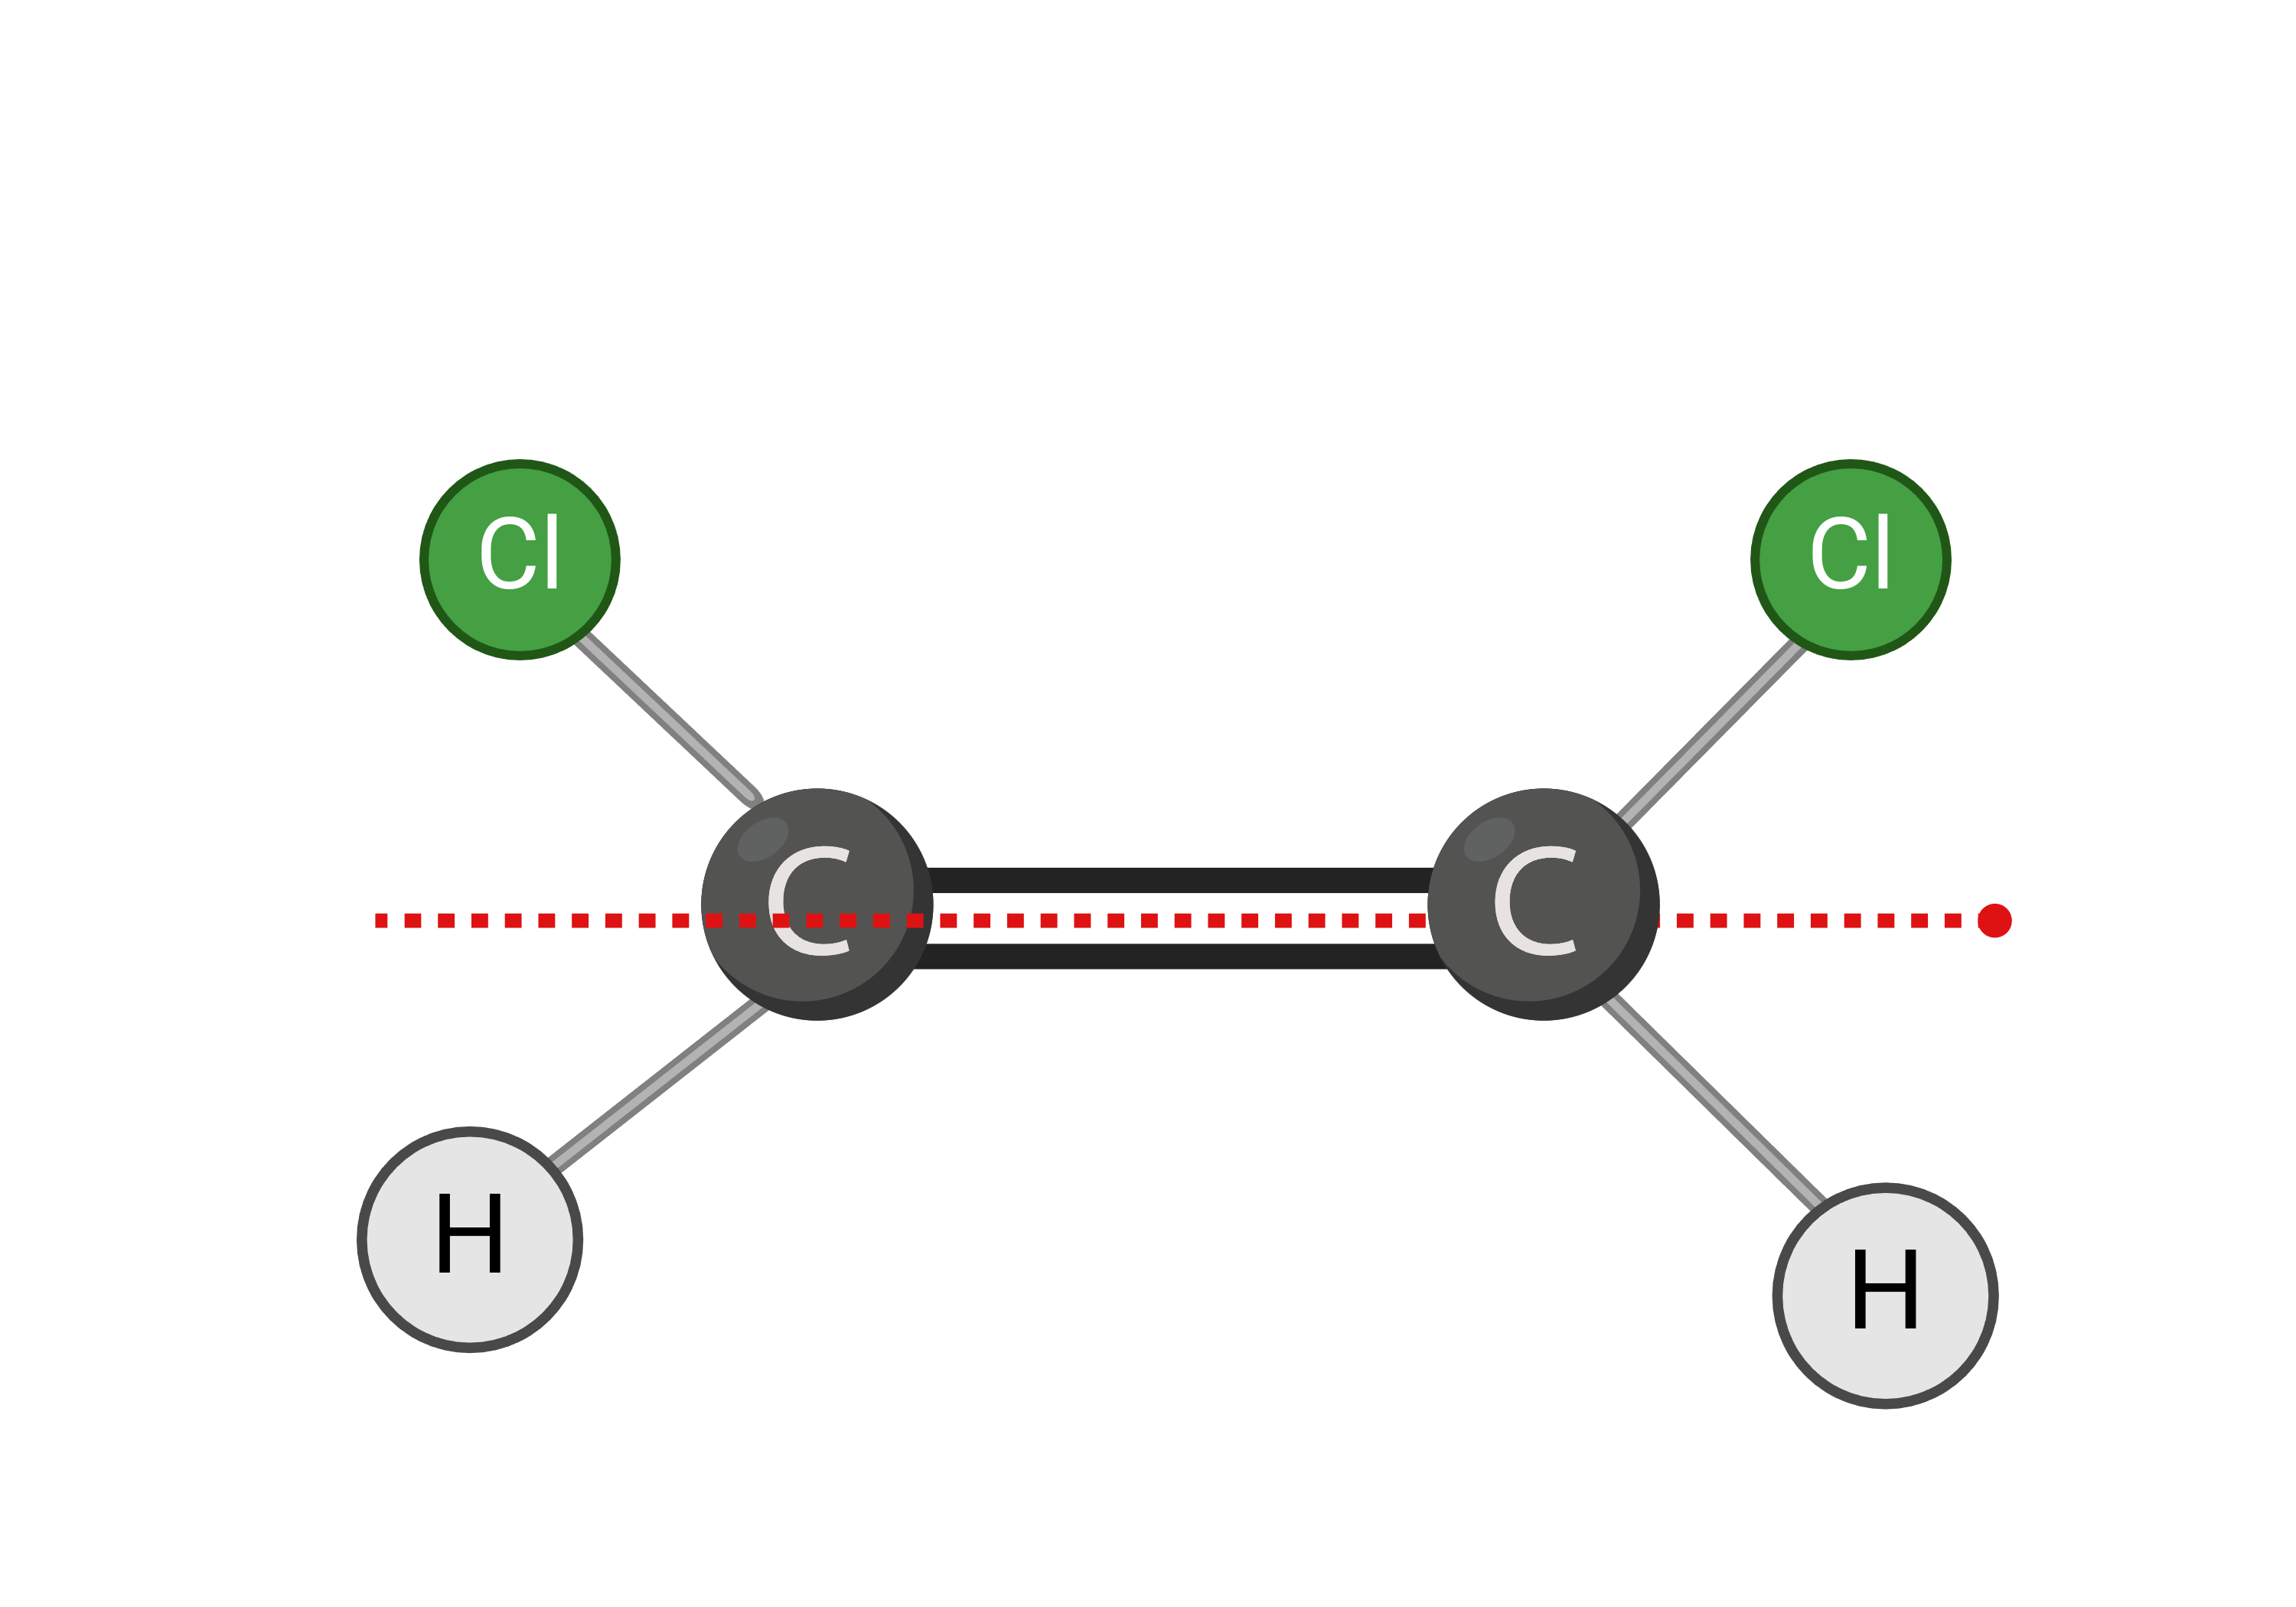
\includegraphics[width=.9\linewidth]{./CIS.png}
\caption{\emph{cis} grupos do mesmo lado. \emph{cis}-1,2-dicloro-eteno}
\end{figure}
\end{column}

\begin{column}{0.4\columnwidth}
\begin{figure}[htbp]
\centering
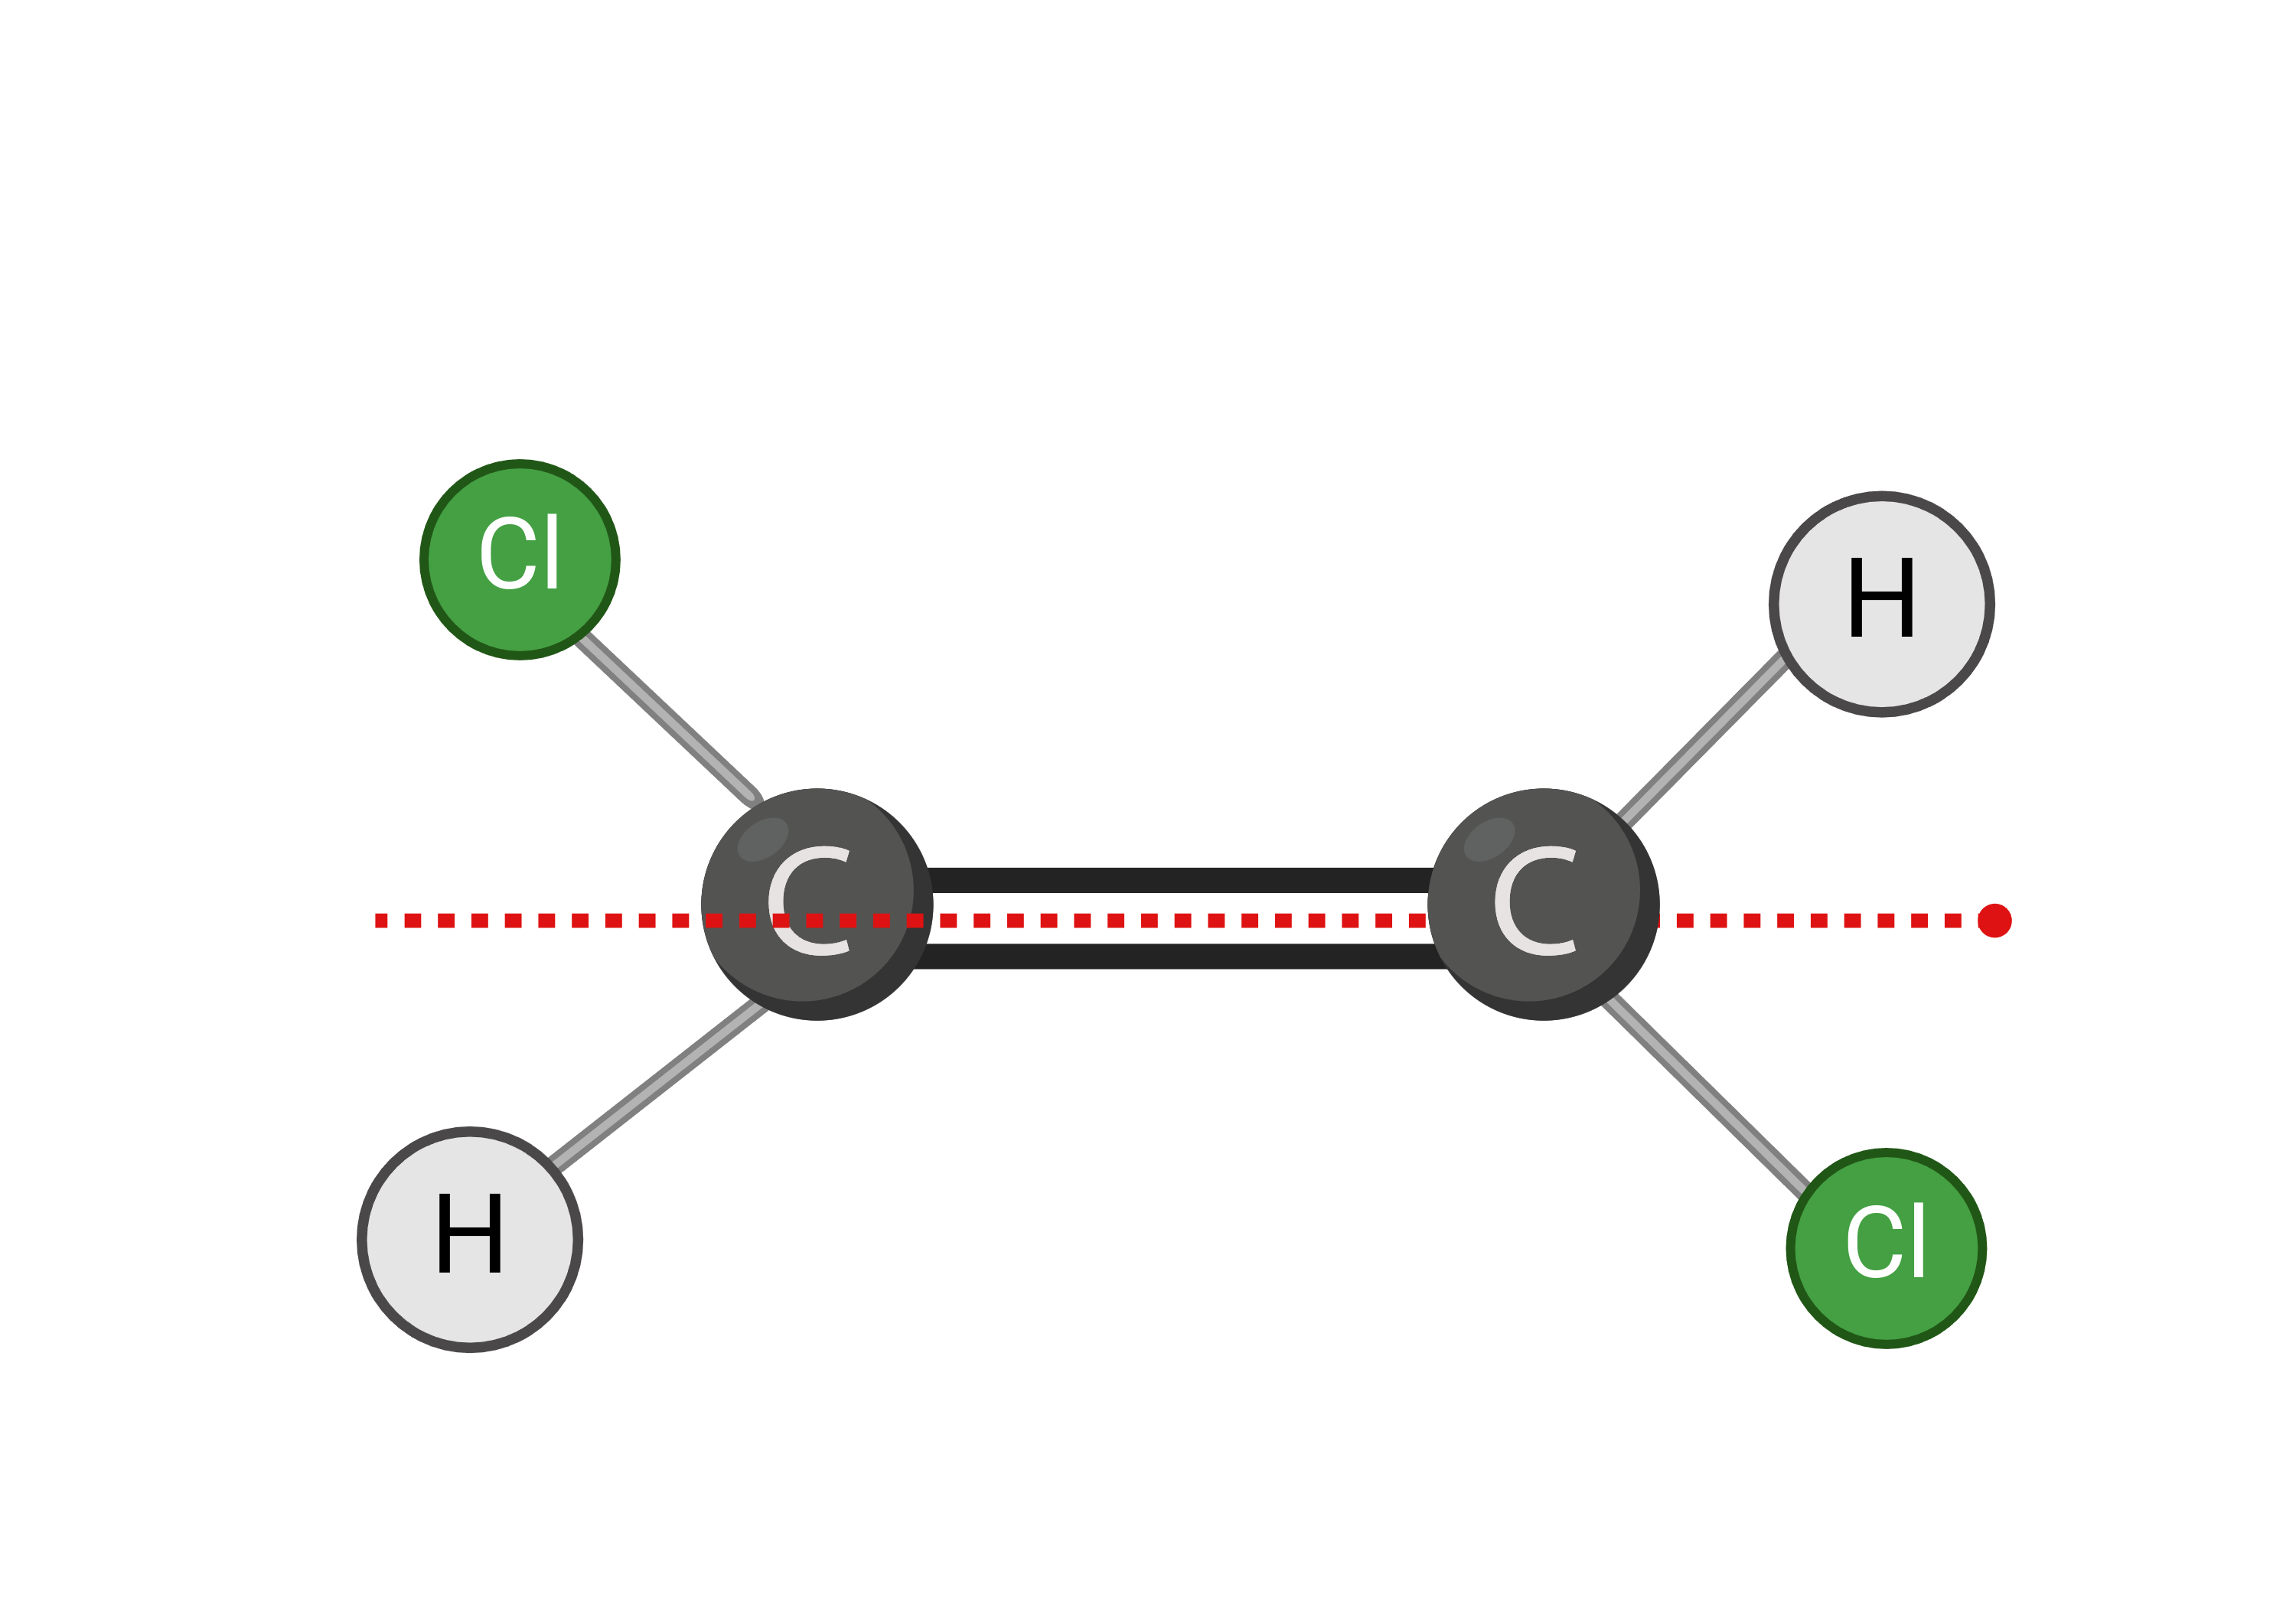
\includegraphics[width=.9\linewidth]{./Trans.png}
\caption{\emph{trans} grupos de lados opostos.  \emph{cis}-1,2-dicloro-eteno}
\end{figure}
\end{column}
\end{columns}
\end{block}
\end{frame}



\begin{frame}[label={sec:org61eab86}]{Isomeria dos  Compostos cíclicos}
\begin{block}{Compostos cíclicos}
\begin{tblr}{ccc}

\schemestart
\chemname{\chemfig{@{a1}H_3C@{a2}>[:330,,2](<:[:225]H)-(<[:30,,,1]@{a3}CH_3@{a4})(<:[:315]H)-[:240](%
-[:120])}}{{\itshape cis}-1,2-dimetilcicloprano} 
\schemestop
\chemmove{
\node[inner sep=2pt,fill=red,fill opacity=0.2, fit=(a1) (a2)]{};
\node[inner sep=2pt,fill=red,fill opacity=0.2, fit=(a3) (a4)]{};
} & \qquad \qquad &
\schemestart
\chemname{\chemfig{@{a1}H_3C@{a2}>[:330,,2](<:[:225]H)-(<[:30]H)(<:[:315,,,1]@{a3}CH_3@{a4})-[:240](%
-[:120])}}{{\itshape trans}-1,2-dimetilcicloprano}
\schemestop
\chemmove{
    \node[inner sep=2pt,fill=red,fill opacity=0.2, fit=(a1) (a2)]{};
    \node[inner sep=2pt,fill=red,fill opacity=0.2, fit=(a3) (a4)]{};
}\\
\end{tblr}



\wedgehasheddash
\begin{tblr}{ccc}
\cyclohexanev{2B==OH;3A==OH} & \cyclohexanev{2SA==H;2SB==OH;3SB==OH;3SA==H} & \cyclohexanev{2SA==H;2SB==OH;3Sd==OH;3Su==H}\\
{\bfseries {\itshape trans}-cicloexan-1,2-diol} & {\bfseries {\itshape cis}-cicloexan-1,2-diol} & {\bfseries {\itshape trans}-cicloexan-1,2-diol}
 \end{tblr}
\end{block}


\begin{block}{Alquenos Dissubstituídos}
\begin{itemize}
\item Os termos \emph{cis} e \emph{trans} são usados apenas para alcenos \alert{dissubstituídos}.
\end{itemize}

\begin{center}
\small
\schemestart
\chemname{\chemfig{H_3C-[:-60]C(-[:-120]H)=C(-[:-60]H)-[:60]CH_3}}{\bfseries{\itshape cis}-but-2-eno}
\qquad
\chemname{\chemfig{H-[:-60]C(-[:-120]H_3C)=C(-[:-60]H)-[:60]CH_3}}{\bfseries{\itshape trans}-but-2-eno}
\qquad
\chemname{\chemfig{H_3CCH_2-[:-60,,3]C(-[:-120]H)=C(-[:-60]H)-[:60]CH_3}}{\bfseries{\itshape cis}-pent-2-eno}
\qquad
\chemname{\chemfig{H-[:-60]C(-[:-120]H_3C)=C(-[:-60]H)-[:60]CH_2CH_3}}{\bfseries{\itshape trans}-pent-2-eno}
\schemestop
\end{center}
\end{block}




\begin{block}{Exemplos}
\begin{question}
\scriptsize\{
(\alert{UERJ}) O ácido linoleico, essencial à dieta humana, apresenta a seguinte fórmula estrutural espacial:

\begin{center}
%\chemfig{-[:330]-[:30]-[:330]-[:30]-[:330]=[:30]-[:330]-[:30]=[:330]-[:30]%
%-[:330]-[:30]-[:330]-[:30]-[:330]-[:30]-[:330](=[:30]O)-[:270]H}
{\scriptsize

\chemfig{OH-[:150,,1](=[:90]O)-[:210]-[:150]-[:210]-[:150]-[:210]-[:150]%
-[:210]-[:150]=[:210]-[:270]-[:210]=[:150]-[:90]-[:150]-[:90]-[:150]-[:90]}
}
\end{center}
Como é possível observar, as ligações duplas presentes nos átomos de carbono 9 e 12 afetam o formato espacial da molécula. As conformações espaciais nessas ligações duplas são denominadas, respectivamente:

\begin{choice}(2)
\choice cis e cis
\choice cis e trans
\choice trans e cis
\choice trans e trans
\end{choice}
\}
\end{question}
\end{block}

\begin{block}{}
\begin{answer}[print=true]
\scriptsize{
Analisando as duas insaturações das moléculas, observa-se que os ligantes não mostrados são átomos de hidrogênio. Em ambas as insaturações, os átomos de hidrogênio estão do mesmo lado da ligação dupla, logo estão em posição \alert{cis}.

\chemfig{OH-[:150,,1](=[:90]O)-[:210]-[:150]-[:210]-[:150]-[:210]-[:150]%
-[:210]-[:150](-[:90]H)=[:210](-[:150]H)-[:270]-[:210](-[:270]H)=[:150](%
-[:210]H)-[:90]-[:150]-[:90]-[:150]-[:90]}
}
\end{answer}
\end{block}
\end{frame}



\begin{frame}[label={sec:org7f9fbec}]{Regra de Cahn–Ingold–Prelog}
\begin{block}{Prefixos E e Z}
\begin{itemize}
\item Para designar alquenos tri e tetrassubstituídos utiliza-se outro sistema de nomenclatura, denominado \alert{E-Z}.
\item No sistema E-Z são examinados os grupos ligados a cada átomo de carbono da dupla ligação e colocados em ordem de prioridade.
\item Os átomos de maior número atômico têm maior prioridade. Ordem decrescente de prioridade:
\end{itemize}

\begin{center}
\schemestart
I > Br > \ch{C$\ell$} > S > F > O > N > C > H
\schemestop
	\chemmove{
	\node[single arrow, draw=black, fill=red8!30, 
	minimum width = 10pt, single arrow head extend=3pt,
	minimum height=10mm, below=1cm of c1,font=\bfseries] {Ordem descrescente de prioridade}; % length of arrow
	}
	\end{center}

\framebreak

\begin{itemize}
\item No caso de átomos de mesmo número atômico, o isótopo de maior número de massa tem maior prioridade:

\begin{tcolorbox}[colback=red!5!white,colframe=red!75!black]
 Hidrogênio \ch{->} \isotope{3,H} > \isotope{2,H} > \isotope{1,H}\\
 Carbono \ch{->} \isotope{14,C} > \isotope{13,C} > \isotope{12,C} 
\end{tcolorbox}

\item Quando os átomos ligados aos carbonos da ligação dupla forem iguais, os números e as massas atômicas dos elementos ligados a esses átomos são usados para realizar o desempate.
\item No sistema \alert{E-Z}, examinam-se os dois átomos ou grupos ligados em cada um dos carbonos da ligação dupla e determina-se a ordem de prioridade de cada um deles.
\item Se os grupos de maior prioridade em cada carbono estiverem do mesmo lado de um plano imaginário passando por esses carbonos, a geometria dessa dupla ligação será designada pela letra Z (do alemão \emph{Zusammen}, \alert{“juntos”}).
\item Se os grupos de maior prioridade em cada carbono estiverem em lados opostos da dupla ligação, a geometria da ligação será designada pela letra E (do alemão \emph{Entgegen}, \alert{“opostos”}).
\end{itemize}

\framebreak


\begin{center}
\schemestart                                           
\chemfig{@{a1}C{\ell}@{a2}-[:-60,1]C(-[:-120]@{a4}F)=C(-[:-60]@{a5}H)-[:60]@{a3}Br}
\schemestop
\end{center}

\begin{itemize}
\item Os átomos ligados ao \alert{C1} são Cl (prioridade 1) e F (prioridade 2) e os ligados ao \alert{C2}, Br (prioridade 1) e H (prioridade 2). Grupos de maior prioridade ligados do mesmo lado da dupla.
\end{itemize}

\vspace{.4cm}
\begin{center}
\schemestart                                           
\chemname[4ex]{\chemfig{@{a1}C{\ell}@{a2}-[:-60,1]C(-[:-120]@{a4}F)=C(-[:-60]@{a5}H)-[:60]@{a3}Br}}{\textcolor{red}{(Z )-2-bromo-1-cloro-1-fluoroeteno}}
\schemestop
\chemmove{
\node[circle, draw, inner sep=2pt,above=.2cm of a1] (label) {1};
\node[circle, draw, inner sep=2pt,above=.2cm of a3] (label) {1};
\node[circle, draw, inner sep=2pt,below=.2cm of a4] (label) {2};
\node[circle, draw, inner sep=2pt,below=.2cm of a5] (label) {2};
}
\end{center}


\framebreak


\begin{center}
\schemestart                                           
\chemname[6ex]{\chemfig{@{a1}H_3C@{a2}-[:-60,1]C(-[:-120]@{a4}H)=C(-[:-60]@{a5}H)-[:60]@{a3}CH_3}}{\bfseries {\itshape Z}-but-2-eno} \qquad \qquad  \qquad 
\chemname[6ex]{\chemfig{@{a7}H_3C@{a7}-[:-60,1]C(-[:-120]@{a8}H)=C(-[:-60]@{a9}CH_3)-[:60]@{a10}H}}{\bfseries {\itshape E}-but-2-eno}
\schemestop
\chemmove{
\node[circle, draw, inner sep=2pt,above=.2cm of a1] (label) {1};
\node[circle, draw, inner sep=2pt,above=.2cm of a3] (label) {1};
\node[circle, draw, inner sep=2pt,below=.2cm of a4] (label) {2};
\node[circle, draw, inner sep=2pt,below=.2cm of a5] (label) {2};
%%%%% MOLECULA 2
\node[circle, draw, inner sep=2pt,above=.33cm of a7] (label) {1};
\node[circle, draw, inner sep=2pt,above=.33cm of a10] (label) {2};
\node[circle, draw, inner sep=2pt,below=.3cm of a8] (label) {2};
\node[circle, draw, inner sep=2pt,below=.3cm of a9] (label) {1};
}

\end{center}


\framebreak

\begin{center}
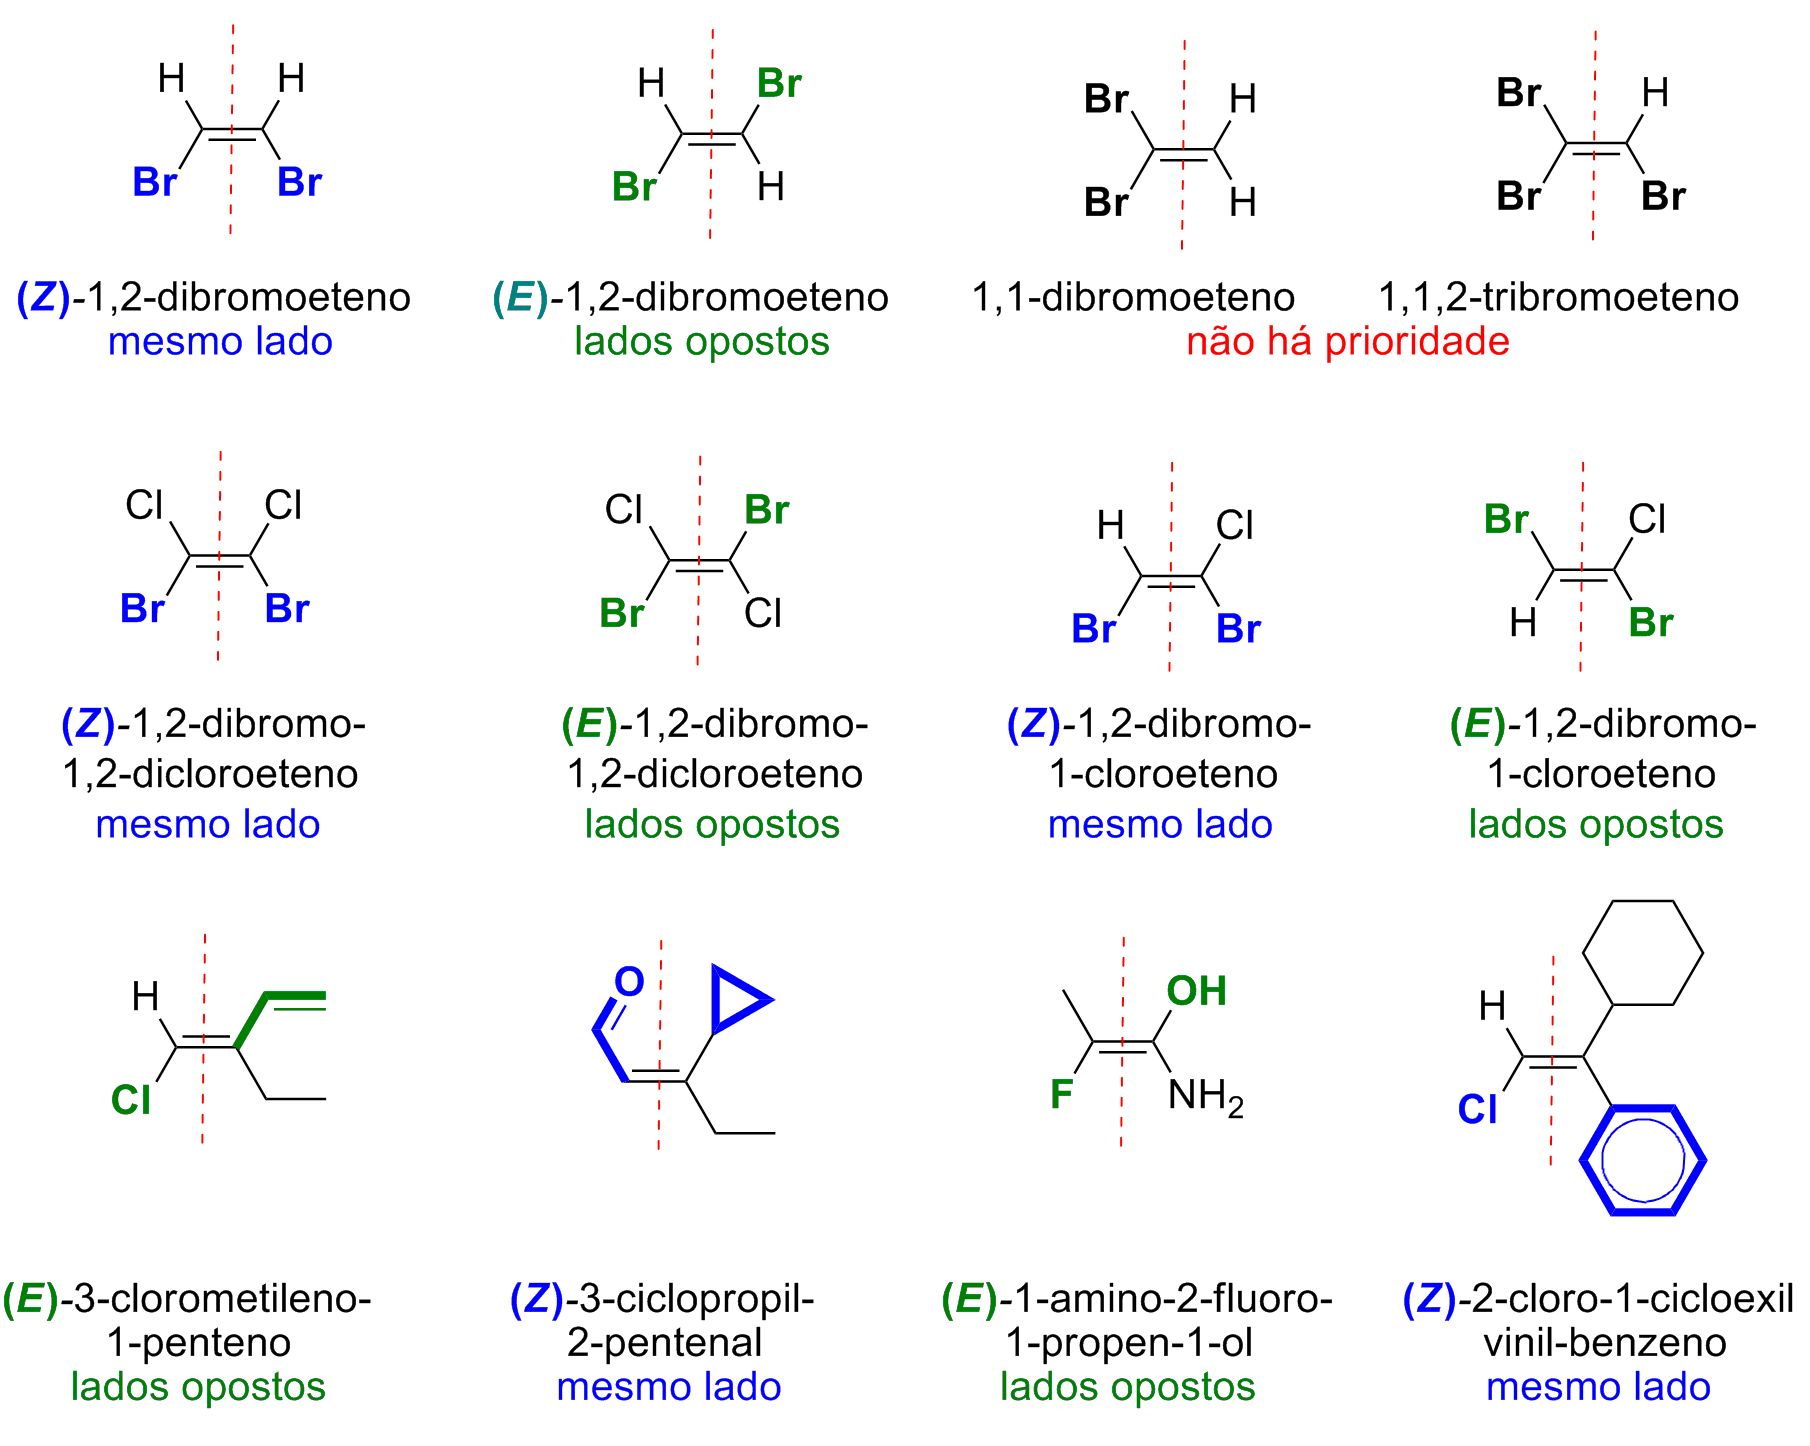
\includegraphics[scale=0.22]{./org_ez.png}
\end{center}
\end{block}
\end{frame}

\begin{frame}[label={sec:org3efc155}]{Isomeria Geométrica com Heteroátomos}
\begin{block}{Isomeria Geométrica com Heteroátomos}
\begin{itemize}
\item Algumas funções que contém ligados a carbono sp\textsuperscript{2}, como as oximas e iminas, possuem geometria definida já que o giro em torno da ligação \(\pi\) possui energia em geral proibitiva. Esses compostos podem ser nomeados seguindo o sistema (\alert{E})-(\alert{Z}) como utilizado em alcenos.
\end{itemize}

\begin{center}
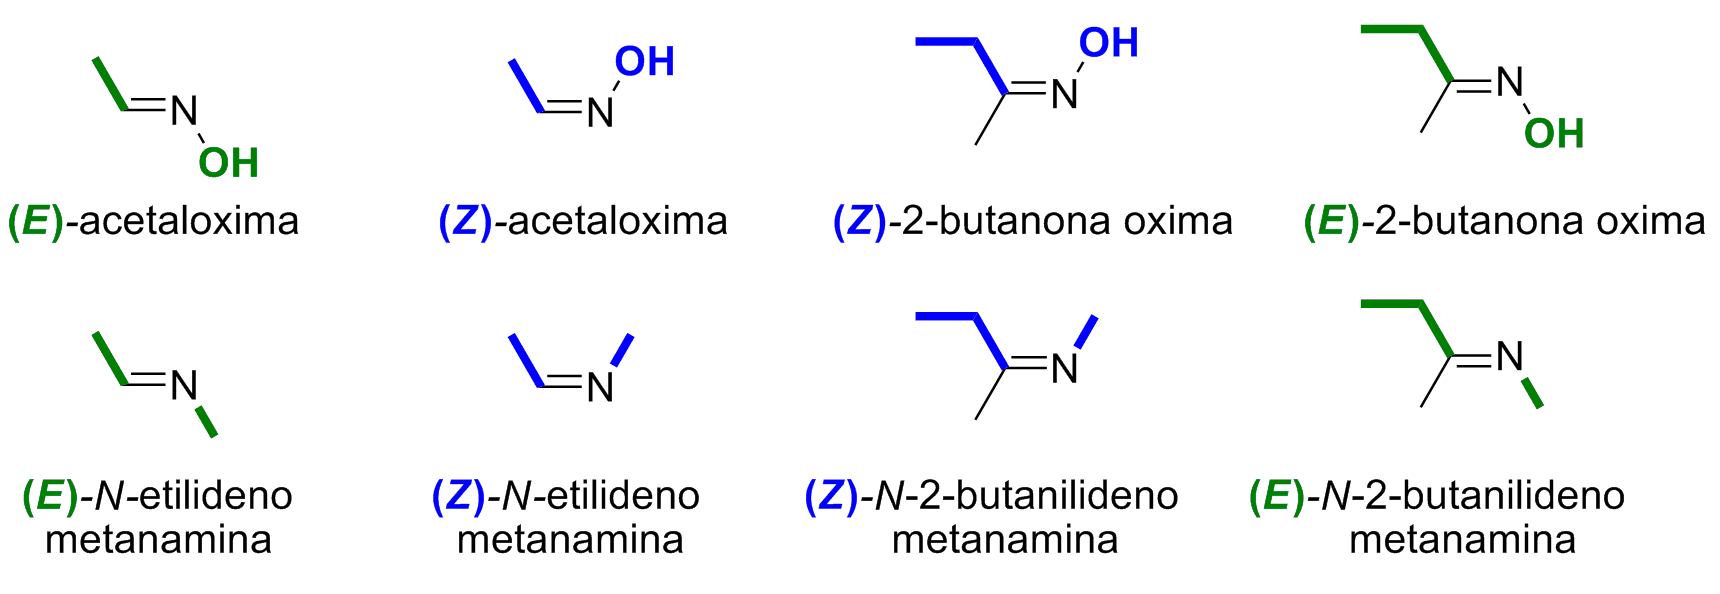
\includegraphics[width=.9\linewidth]{./org_ez_hetero.png}
\end{center}
\end{block}







\begin{block}{Fim da Aula}
\begin{tikzpicture}
\node[graduate,sword, minimum size=1cm]{ \bfseries Bons Estudos !!!!};
\end{tikzpicture}
\begin{center}
\begin{tabular}{ccc}
Download Aula  \\%& & Lista de Exercícios \\
 \qrcode[height=2in]{https://github.com/fabinholima/AulaQuimicaPDF/blob/main/QO/Isomeria/Isomeria_Geometrica.pdf} \\  %& & \qrcode[height=2in]{https://mark.nl.tab.digital/s/6kSsDYwW4icCK9X}\\
 \end{tabular}
 \end{center}
\end{block}
\end{frame}
\end{document}
